%%%%%%%%%%%%%%%%%%%%%%%%%%%%%%%%%%%%%%%%%%%%%%%%%%%%%%%%%%%%%%%%%%%%%
%
% Complete documentation on the extended LaTeX markup used for Insight
% documentation is available in ``Documenting Insight'', that is part
% of the standard documentation for Insight.  It may be found online
% at:
%
%                    https://www.itk.org
%
%%%%%%%%%%%%%%%%%%%%%%%%%%%%%%%%%%%%%%%%%%%%%%%%%%%%%%%%%%%%%%%%%%%%%

\documentclass{InsightSoftwareGuide}

\usepackage[dvips]{graphicx}
\usepackage{times}
\usepackage{color}
\usepackage{listings}
\usepackage{minted}
\usepackage{setspace}
\usepackage{hyphenat}
\usepackage[toc,page]{appendix}
\usepackage{verbatim}
\usepackage{imakeidx}

\usepackage{draftwatermark}
%\usepackage[firstpage]{draftwatermark}
\SetWatermarkText{DRAFT-ITK}%default is DRAFT
\SetWatermarkLightness{0.90}%default is 0.8
\SetWatermarkScale{0.8}%default is 1.2

%\allowhyphens

\lstnewenvironment{itklisting}
{\singlespacing\lstset{language=C++}}
{}

\definecolor{ltgray}{rgb}{0.97,0.97,0.97}
\usemintedstyle{emacs}

\lstset{
         basicstyle=\footnotesize\ttfamily, % Standardschrift
         %numbers=left,               % Ort der Zeilennummern
         numberstyle=\tiny,          % Stil der Zeilennummern
         %stepnumber=2,               % Abstand zwischen den Zeilennummern
         numbersep=2pt,              % Abstand der Nummern zum Text
         tabsize=2,                  % Groesse von Tabs
         extendedchars=true,         %
         breaklines=true,            % Zeilen werden Umgebrochen
         keywordstyle=\color{red},
 %    frame=b,
 %        keywordstyle=[1]\textbf,    % Stil der Keywords
 %        keywordstyle=[2]\textbf,    %
 %        keywordstyle=[3]\textbf,    %
 %        keywordstyle=[4]\textbf,   \sqrt{\sqrt{}} %
         stringstyle=\color{black}\ttfamily, % Farbe der String
         showspaces=false,           % Leerzeichen anzeigen ?
         showtabs=false,             % Tabs anzeigen ?
         xleftmargin=17pt,
         framexleftmargin=17pt,
         framexrightmargin=5pt,
         framexbottommargin=4pt,
         backgroundcolor=\color{ltgray},
         showstringspaces=false      % Leerzeichen in Strings anzeigen ?
 }

 \lstloadlanguages{% Check Dokumentation for further languages ...
         %[Visual]Basic
         %Pascal
         %C
         C++
         %XML
         %HTML
         %Java
 }
%\DeclareCaptionFont{blue}{\color{blue}}

%\captionsetup[lstlisting]{singlelinecheck=false, labelfont={blue}, textfont={blue}}
\usepackage{caption}
\DeclareCaptionFont{white}{\color{white}}
\DeclareCaptionFormat{listing}{\colorbox[cmyk]{0.43, 0.35, 0.35,0.01}{\parbox{\textwidth}{\hspace{15pt}#1#2#3}}}
\captionsetup[lstlisting]{format=listing,labelfont=white,textfont=white, singlelinecheck=false, margin=0pt, font={bf,footnotesize}}

\newif\ifitkFullVersion
\itkFullVersiontrue
%\itkFullVersionfalse


%%%%%%%%%%%%%%%%%%%%%%%%%%%%%%%%%%%%%%%%%%%%%%%%%%%%%%%%%%%%%%%%%%%
%
%
%   Load configuration parameters prepared by CMake
%
%
%%%%%%%%%%%%%%%%%%%%%%%%%%%%%%%%%%%%%%%%%%%%%%%%%%%%%%%%%%%%%%%%%%%

\input{SoftwareGuideConfiguration.tex}

%%%%%%%%%%%%%%%%%%%%%%%%%%%%%%%%%%%%%%%%%%%%%%%%%%%%%%%%%%%%%%%%%%
%
%  hyperref should be the last package to be loaded.
%
%%%%%%%%%%%%%%%%%%%%%%%%%%%%%%%%%%%%%%%%%%%%%%%%%%%%%%%%%%%%%%%%%%
\ifitkPrintedVersion
\usepackage[dvips,
pdftitle={ITK Software Guide},
pdfauthor={Hans Johnson and Luis Ib'{a}~{n}ez and Matthew McCormick and the Insight Software Consortium},
pdfsubject={Medical Image Segmentation and Registration Toolkit}
pdfkeywords={Registration,Segmentation,Guide},
pdfpagemode={UseOutlines},
bookmarks,bookmarksopen,
pdfstartview={FitH},
backref,
colorlinks,linkcolor={black},citecolor={black},urlcolor={black},
]{hyperref}
\else
\usepackage[dvips,
pdftitle={ITK Software Guide},
pdfauthor={Hans Johnson and Luis Ib'{a}~{n}ez and Matthew McCormick and the Insight Software Consortium},
pdfsubject={Medical Image Segmentation and Registration Toolkit},
pdfkeywords={Registration,Segmentation,Guide},
pdfpagemode={UseOutlines},
bookmarks,bookmarksopen,
pdfstartview={FitH},
backref,
colorlinks,linkcolor={blue},citecolor={blue},urlcolor={blue},
]{hyperref}
\fi

%%%%%%%%%%%%%%%%%%%%%%%%%%%%%%%%%%%%%%%%%%%%%%%%%%%%%%%%%%%%%%%%%%%
%
%
%           The Insight Toolkit Software Guide
%
%
%%%%%%%%%%%%%%%%%%%%%%%%%%%%%%%%%%%%%%%%%%%%%%%%%%%%%%%%%%%%%%%%%%%

\author{Hans J. Johnson, Matthew M. McCormick, Luis Ib\'{a}\~{n}ez, and the \emph{Insight Software Consortium}}

\authoraddress{
  \url{http://itk.org}\\
  Email: \email{community@itk.org}
}

\date{\today}

% actually write the .idx file
\makeindex

\setcounter{tocdepth}{3}



\title{The ITK Software Guide\\Book 2: Design and Functionality\\ \emph{Updated for ITK version
\ITKVERSIONMAJORMINOR}}


%%%%%%%%%%%%%%%%%%%%%%%%%%%%%%%%%%%%%%%%%%%%%%%%%%%%%%%%%%%%%%%%%%%
%
%           Begin Document
%
%%%%%%%%%%%%%%%%%%%%%%%%%%%%%%%%%%%%%%%%%%%%%%%%%%%%%%%%%%%%%%%%%%%

\begin{document}

\ifitkPrintedVersionFirstPage

  \begin{minipage}[t][3cm][b]{\textwidth}
  \rule{14cm}{1pt}
  \end{minipage}

  \begin{minipage}[t][3cm][b]{\textwidth}
  \Huge
  The ITK Software Guide
  \par
  \Large
  Book 2: Design and Functionality\\
  \normalsize
  \par
  \emph{Updated for version \ITKVERSIONMAJORMINOR}\\

  \end{minipage}

  %\hfill
\begin{minipage}[t][6cm][b]{0.6\textwidth}
\Large
\renewcommand{\baselinestretch}{1.5}
Hans J. Johnson\\
Matthew McCormick \\
Luis Ib\'{a}\~{n}ez\\
and the \emph{Insight Software Consortium}
\normalsize
\end{minipage}


\begin{minipage}[t][2cm][b]{\textwidth}
\rule{14cm}{1pt}
\end{minipage}

\newpage

\begin{minipage}[t][4cm][b]{\textwidth}
\begin{center}
\includegraphics[width=0.5\textwidth]{Kitware-logo-medium-res.eps}
\end{center}
\par
\begin{center}
\large

\copyright \the\year \; Kitware, Inc. \emph{(cover, preface, postface)}\\
\copyright \the\year \; Insight Software Consortium \emph{(main text body)}\\
Published by Kitware, Inc. \texttt{http://www.kitware.com}
\normalsize
\end{center}
\end{minipage}


\begin{minipage}[t][2.25cm][b]{\textwidth}
\begin{center}
An electronic version of this document is available from
\texttt{https://itk.org}.
\end{center}
\begin{tabular}{p{.9\textwidth}}
This work is licensed under a Creative Commons Attribution 3.0 Unported License.
\begin{center}
\includegraphics[width=3.4cm]{cc-by.eps}
\end{center}\\
\end{tabular}
\end{minipage}


\begin{minipage}[t][2.5cm][b]{\textwidth}
\begin{center}
This project has been funded in whole or in part with Federal funds from the
National Institutes of Health (NLM, NIDCR, NIMH, NEI, NINDS, NIDCD, NCI), the
NSF, and the DoD (TATRC). Funding has primarily come under the direction of the
National Library of Medicine, National Institutes of Health, under numerous
contracts. Recently, the major revision to the toolkit, ITKv4, was made
possible by NLM directed funds from the American Reinvestment and Recovery Act
(ARRA).
\end{center}
\end{minipage}


\begin{minipage}[t][1.0cm][b]{\textwidth}
\begin{center}
All product names mentioned herein are the trademarks of their respective
owners.
\end{center}
\end{minipage}


\begin{minipage}[t][2.7cm][b]{\textwidth}
\begin{center}
Document created with \LaTeX{}, using CMake as
configuration manager, with a Python script to extract examples from the
\code{ITK/Examples} directory. All code in this document compiled at
the time of publication.
\end{center}
\end{minipage}

  %\begin{minipage}[t][1.0cm][b]{\textwidth}
\begin{center}
Printed and produced in the United States of America.\\
\textbf{ISBN 978-1-930934-36-8}
\end{center}
\end{minipage}


\fi

\maketitle
\ifitkPrintedVersion
  \newgeometry{inner=3cm,outer=2cm,bottom=1.5cm}
\fi

\frontmatter

\hyperbaseurl{https://www.itk.org/Insight}

\ifitkPrintedVersion
  \hfill
\begin{minipage}[t][6cm][b]{0.6\textwidth}
\Large
\renewcommand{\baselinestretch}{1.5}
Hans J. Johnson\\
Matthew McCormick \\
Luis Ib\'{a}\~{n}ez\\
and the \emph{Insight Software Consortium}
\normalsize
\end{minipage}


\begin{minipage}[t][2cm][b]{\textwidth}
\rule{14cm}{1pt}
\end{minipage}

\newpage

\begin{minipage}[t][4cm][b]{\textwidth}
\begin{center}
\includegraphics[width=0.5\textwidth]{Kitware-logo-medium-res.eps}
\end{center}
\par
\begin{center}
\large

\copyright \the\year \; Kitware, Inc. \emph{(cover, preface, postface)}\\
\copyright \the\year \; Insight Software Consortium \emph{(main text body)}\\
Published by Kitware, Inc. \texttt{http://www.kitware.com}
\normalsize
\end{center}
\end{minipage}


\begin{minipage}[t][2.25cm][b]{\textwidth}
\begin{center}
An electronic version of this document is available from
\texttt{https://itk.org}.
\end{center}
\begin{tabular}{p{.9\textwidth}}
This work is licensed under a Creative Commons Attribution 3.0 Unported License.
\begin{center}
\includegraphics[width=3.4cm]{cc-by.eps}
\end{center}\\
\end{tabular}
\end{minipage}


\begin{minipage}[t][2.5cm][b]{\textwidth}
\begin{center}
This project has been funded in whole or in part with Federal funds from the
National Institutes of Health (NLM, NIDCR, NIMH, NEI, NINDS, NIDCD, NCI), the
NSF, and the DoD (TATRC). Funding has primarily come under the direction of the
National Library of Medicine, National Institutes of Health, under numerous
contracts. Recently, the major revision to the toolkit, ITKv4, was made
possible by NLM directed funds from the American Reinvestment and Recovery Act
(ARRA).
\end{center}
\end{minipage}


\begin{minipage}[t][1.0cm][b]{\textwidth}
\begin{center}
All product names mentioned herein are the trademarks of their respective
owners.
\end{center}
\end{minipage}


\begin{minipage}[t][2.7cm][b]{\textwidth}
\begin{center}
Document created with \LaTeX{}, using CMake as
configuration manager, with a Python script to extract examples from the
\code{ITK/Examples} directory. All code in this document compiled at
the time of publication.
\end{center}
\end{minipage}

  \begin{minipage}[t][1.0cm][b]{\textwidth}
\begin{center}
Printed and produced in the United States of America.\\
\textbf{ISBN 978-1-930934-36-8}
\end{center}
\end{minipage}

\fi

%%%%%%%%%%%%%%%%%%%%%%%%%%%%%%%%%%%%%%%%%%
%
%  Page with Quote and ITK Logo
%
%
%%%%%%%%%%%%%%%%%%%%%%%%%%%%%%%%%%%%%%%%%%
\cleardoublepage

\begin{minipage}[t][10cm][b]{\textwidth}
\center
\includegraphics[width=0.5\textwidth]{itkLogo.eps}
\large
\begin{center}
\emph{The purpose of computing is Insight, not numbers.}\\
\end{center}
\hspace{8cm} Richard Hamming
\normalsize
\end{minipage}



%%%%%%%%%%%%%%%%%%%%%%%%%%%%%%%%%%%%%%%%%%%%%%
%
% remove headings from the following material
\pagestyle{plain}
%
%%%%%%%%%%%%%%%%%%%%%%%%%%%%%%%%%%%%%%%%%%%%%%


\ifitkPrintedVersion
  % We want this material to fit on two pages
\small

\chapter*{About the Cover}

The cover image consists of a photograph of ABS plastic anatomical objects
printed with a MakerBot Replicator 2X 3D printer. Mesh STL files were generated from the images with VTK.

\begin{description}

\item [Skull.]
Given that the origins of ITK are with the Visible Human Project, it is
appropriate that the skull was derived from the Visible Woman dataset. The
skull was segmented with ITK from the Visible Woman head CT images with simple
thresholding\footnote{\url{https://github.com/XiaoxiaoLiu/3D-printing}}.

\item[Brain.]
The brain model was segmented with ITK as described in the open science
publication:
\begin{quote}
McCormick M, Liu X, Jomier J, Marion C and Ibanez L. ITK:
enabling reproducible research and open science. Front. Neuroinform. 8:13.
2014. doi: 10.3389/fninf.2014.00013
\end{quote}

\end{description}

\normalsize

\fi

\chapter*{Abstract}
\noindent
The Insight Toolkit \href{http://itk.org}{(ITK)} is an open-source
software toolkit for performing registration and
segmentation. \emph{Segmentation} is the process of identifying and
classifying data found in a digitally sampled
representation. Typically the sampled representation is an image
acquired from such medical instrumentation as CT or MRI
scanners. \emph{Registration} is the task of aligning or developing
correspondences between data. For example, in the medical environment,
a CT scan may be aligned with a MRI scan in order to combine the
information contained in both.

ITK is a cross-platform software. It uses a build environment known as
\href{http://cmake.org}{CMake} to manage platform-specific project
generation and compilation process in a platform-independent way. ITK is
implemented in C++. ITK's implementation style employs generic programming,
which involves the use of templates to generate, at compile-time, code that can
be applied \emph{generically} to any class or data-type that supports the
operations used by the template. The use of C++ templating means that the code
is highly efficient and many issues are discovered at compile-time, rather than
at run-time during program execution. It also means that many of ITK's
algorithms can be applied to arbitrary spatial dimensions and pixel types.

An automated wrapping system integrated with ITK generates an interface between
C++ and a high-level programming language \href{http://www.python.org}{Python}.
This enables rapid prototyping and faster exploration of ideas by shortening the
edit-compile-execute cycle. In addition to automated
wrapping, the \href{http://www.itk.org/Wiki/SimpleITK}{SimpleITK} project
provides a streamlined interface to ITK that is available for C++, Python, Java,
CSharp, R, Tcl and Ruby.

Developers from around the world can use, debug, maintain, and extend the
software because ITK is an open-source project. ITK uses a
model of software development known as Extreme
Programming. Extreme Programming collapses the usual software development
methodology into a simultaneous iterative process of
design-implement-test-release. The key features of Extreme Programming
are communication and testing. Communication among the members of the
ITK community is what helps manage the rapid evolution of the
software. Testing is what keeps the software stable. An
extensive testing process supported by the system known as
\href{http://open.cdash.org/index.php?project=Insight}{CDash}
measures the quality of ITK code on a daily basis. The ITK Testing Dashboard is
updated continuously, reflecting the quality of the code at any moment.

The most recent version of this document is available online at
\url{http://itk.org/ItkSoftwareGuide.pdf}.

This book is a guide to developing software with ITK; it is the second of two
companion books. This book covers detailed design and functionality for
reading and writing images, filtering, registration, segmentation, and
performing statistical analysis. The first book covers building and installation, general
architecture and design, as well as the process of contributing in the ITK
community.

\chapter*{Contributors}
\noindent

The Insight Toolkit \href{http://www.itk.org}{(ITK)} has been created by the
efforts of many talented individuals and prestigious organizations. It is also
due in great part to the vision of the program established by Dr. Terry Yoo
and Dr. Michael Ackerman at the National Library of Medicine.

This book lists a few of these contributors in the following paragraphs. Not
all developers of ITK are credited here, so please visit the Web pages at
\href{http://www.itk.org/HTML/About.htm}{http://www.itk.org/HTML/About.htm}
for the names of additional contributors, as well as checking the GIT source
logs for code contributions.

The following is a brief description of the contributors to this software
guide and their contributions.


{\bf Luis Ib\'{a}\~{n}ez} is principal author of this text.
He assisted in the design and layout of the text, implemented the bulk of
the \LaTeX{} and CMake build process, and was responsible for the bulk of
the content. He also developed most of the example code found in the
\code{Insight/Examples} directory.

{\bf Will Schroeder} helped design and establish the organization
of this text and the \code{Insight/Examples} directory. He is principal
content editor, and has authored several chapters.

{\bf Lydia Ng} authored the description for the registration framework
and its components, the section on the multiresolution framework, and
the section on deformable registration methods. She also edited the
section on the resampling image filter and the sections on various
level set segmentation algorithms.

{\bf Joshua Cates} authored the iterators chapter and the text and examples
describing watershed segmentation. He also co-authored the level-set
segmentation material.

{\bf Jisung Kim} authored the chapter on the statistics framework.

{\bf Julien Jomier} contributed the chapter on spatial objects and examples on
model-based registration using spatial objects.

{\bf Karthik Krishnan} reconfigured the process for automatically generating
images from all the examples. Added a large number of new examples and updated
the Filtering and Segmentation chapters for the second edition.

{\bf Stephen Aylward} contributed material describing spatial objects and
their application.

{\bf Tessa Sundaram} contributed the section on deformable registration using
the finite element method.

{\bf YinPeng Jin} contributed the examples on  hybrid segmentation methods.

{\bf Celina Imielinska} authored the section describing the principles of
hybrid segmentation methods.

{\bf Mark Foskey} contributed the examples on the
AutomaticTopologyMeshSource class.

{\bf Mathieu Malaterre} contributed the entire section on the description and
use of DICOM readers and writers based on the GDCM library. He also contributed
an example on the use of the VTKImageIO class.

{\bf Gavin Baker} contributed the section on how to write composite filters.
Also known as minipipeline filters.

Since the software guide is generated in part from the ITK source code
itself, many ITK developers have been involved in updating and
extending the ITK documentation.  These include {\bf David Doria},
{\bf Bradley Lowekamp}, {\bf Mark Foskey}, {\bf Ga\"{e}tan Lehmann},
{\bf Andreas Schuh}, {\bf Tom Vercauteren}, {\bf Cory Quammen}, {\bf Daniel Blezek},
{\bf Paul Hughett}, {\bf Matthew McCormick}, {\bf Josh Cates}, {\bf Arnaud Gelas},
{\bf Jim Miller}, {\bf Brad King}, {\bf Gabe Hart}, {\bf Hans Johnson}.

{\bf Hans Johnson}, {\bf Kent Williams}, {\bf Constantine Zakkaroff}, {\bf
Xiaoxiao Liu}, {\bf Ali Ghayoor}, and {\bf Matthew McCormick} updated
the documentation for the initial ITK version 4 release.




%%%%%%%%%%%%%%%%%%%%%%%%%%%%%%%%%%%%%%%%%%%%%%%%%%%%%%%%%
%
% Insert Table of Contents; List of Figures and Tables
%
%%%%%%%%%%%%%%%%%%%%%%%%%%%%%%%%%%%%%%%%%%%%%%%%%%%%%%%%%


%%%%%%%%%%%%%%%%%%%%%%%%%%%%%%%%%%%%%%%%%%%%%%
%
% enable headings from the following material
\pagestyle{normal}
%
%%%%%%%%%%%%%%%%%%%%%%%%%%%%%%%%%%%%%%%%%%%%%%
\small
\tableofcontents
\listoffigures
\listoftables
\normalsize


%%%%%%%%%%%%%%%%%%%%%%%%%%%%%%%%%%%%%%%%%
%
% Begin technical content
%
%%%%%%%%%%%%%%%%%%%%%%%%%%%%%%%%%%%%%%%%%

\mainmatter



\chapter{Reading and Writing Images}
\label{sec:IO}

This chapter describes the toolkit architecture supporting reading and
writing of images to files. ITK does not enforce any particular file format,
instead, it provides a structure supporting a variety of formats that can
be easily extended by the user as new formats become available.

We begin the chapter with some simple examples of file I/O.

\section{Basic Example}
\label{sec:ImagReadWrite}
\input{ImageReadWrite.tex}

To better understand the IO architecture, please refer to Figures 
\ref{fig:ImageIOCollaborationDiagram}, 
\ref{fig:ImageIOFactoriesUseCases}, and
\ref{fig:ImageIOFactoriesClassDiagram}. 

\begin{figure}
\center
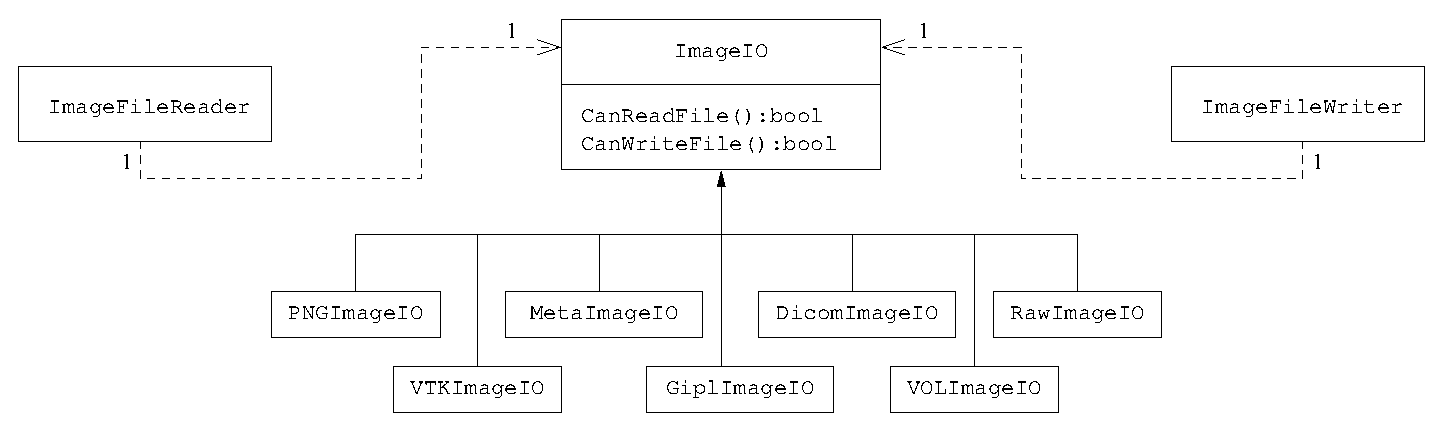
\includegraphics[width=\textwidth]{ImageIOCollaborationDiagram.eps}
\itkcaption[Collaboration diagram of the ImageIO classes]{Collaboration diagram
of the ImageIO classes.} \label{fig:ImageIOCollaborationDiagram}
\end{figure}

\begin{figure}
\center
\includegraphics[width=\textwidth]{ImageIOFactoriesUseCases.eps}
\itkcaption[Use cases of ImageIO factories] {Use cases of ImageIO factories.}
\label{fig:ImageIOFactoriesUseCases}
\end{figure}

\begin{figure}
\center
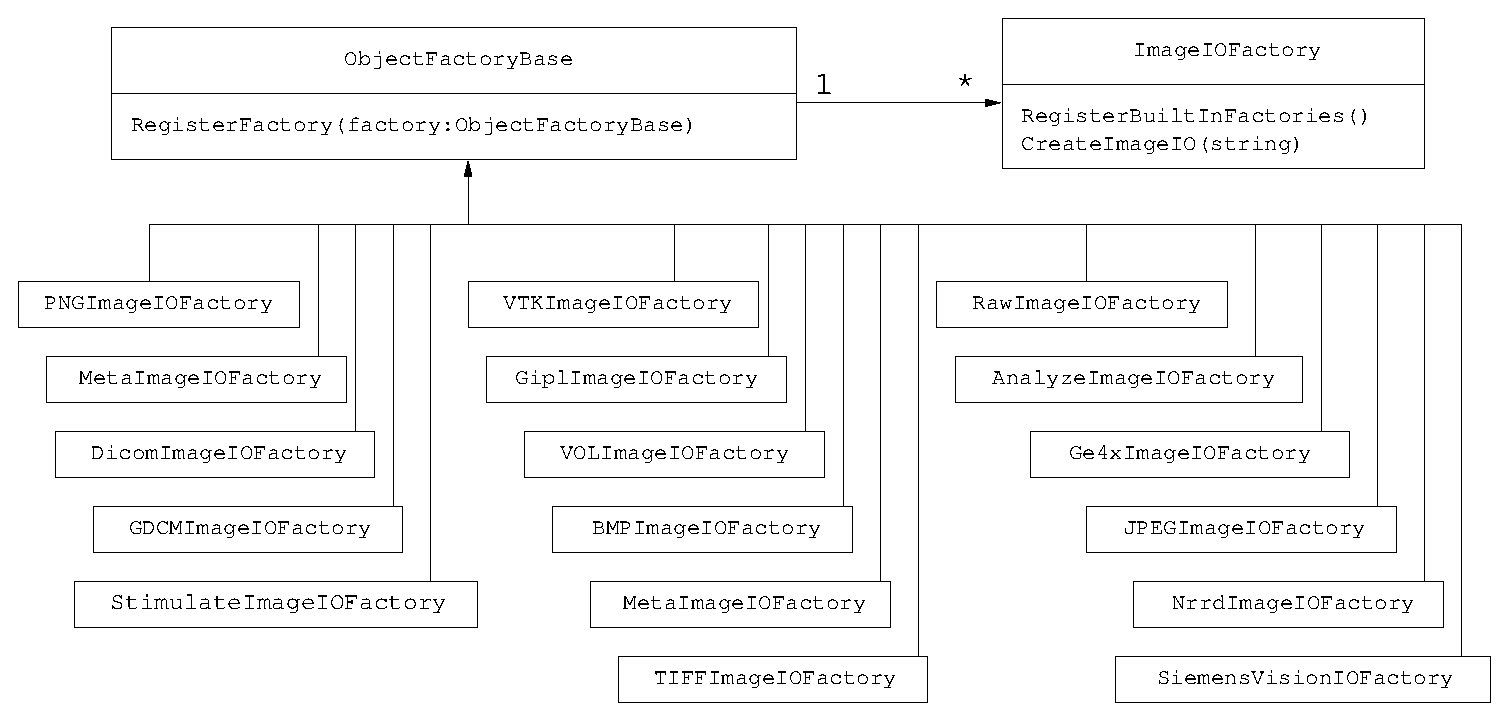
\includegraphics[width=\textwidth]{ImageIOFactoriesClassDiagram.eps}
\itkcaption[Class diagram of ImageIO factories] {Class diagram of the ImageIO
factories.}
\label{fig:ImageIOFactoriesClassDiagram}
\end{figure}

\section{Reading and Writing RGB Images}
\label{sec:RGBImagReadWrite}
\input{RGBImageReadWrite.tex}

\section{Reading, Casting and Writing Images}
\label{sec:ImagReadCastWrite}
\input{ImageReadCastWrite.tex}

\section{Extracting Regions}
\label{sec:ImagReadRegionOfInterestWrite}
\input{ImageReadRegionOfInterestWrite.tex}

\section{Extracting Slices}
\label{sec:ImagReadExtractWrite}
\input{ImageReadExtractWrite.tex}

\section{Reading and Writing Vector Images}
\label{sec:VectorImagReadWrite}

\input{CovariantVectorImageWrite.tex}

Let's now take the image that we just created and read it into another program.

\input{CovariantVectorImageRead.tex}


\section{Extracting Components from Vector Images}
\label{sec:VectorImageExtractComponent}
\input{CovariantVectorImageExtractComponent.tex}

\section{Reading Image Series}
\label{sec:ReadingImageSeries}
\input{ImageSeriesReadWrite.tex}
\input{RGBImageSeriesReadWrite.tex}


\section{Writing Image Series}
\label{sec:WritingImageSeries}
\input{ImageReadImageSeriesWrite.tex}

\section{Reading and Writing DICOM Images}
\label{sec:ReadingDicomImageSeries2}

% Small intro to DICOM file format

\subsection{Foreword}
ACR (the American College of Radiology) and NEMA (the National Electrical Manufacturers Association)
formed a joint committee to develop a Standard for Digital Imaging and COmmunications in Medicine (DICOM).
This DICOM Standard was developed according to the NEMA Procedures. This Standard is developed in liaison with other Standardization Organizations such as CEN TC251, JIRA including IEEE, HL7 and ANSI USA as reviewers.

With the introduction of computed tomography (CT) followed by other digital diagnostic imaging
modalities in the 1970's, and the increasing use of computers in clinical applications, the American
College of Radiology (ACR) and the National Electrical Manufacturers Association (NEMA) recognized
the emerging need for a standard method for transferring images and associated information between
devices manufactured by various vendors. These devices produce a variety of digital image formats.

DICOM is a comprehensive set of standards for handling, storing and transmitting information in medical
imaging. It includes both a file format definition as well as a network communication protocol.
DICOM was developed to enable integration of scanners, servers, workstations and network hardware from
multiple vendors into a picture archiving and communication system.

DICOM files consist of a header with standardized (See Insight/Utilities/gdcm/Dict/dicomV3.dic) as well 
as free-form fields and a body of image data. A single DICOM file can contain one or more frames, 
allowing storage of volumes or animations. Image data can be compressed using a variety of standards,
including JPEG, LZW and Run-length encoding (RLE).

The DICOM Standard is an evolving standard and it is maintained in accordance with the Procedures of
the DICOM Standards Committee. Proposals for enhancements are forthcoming from the DICOM
Committee member organizations based on input from users of the Standard. These proposals are
considered for inclusion in future editions of the Standard. A requirement in updating the Standard is to
maintain effective compatibility with previous editions. An entire newsgroup is dedicated to this: 
newsgroup://comp.protocols.dicom.

For a more detailed description of the DICOM standard see~\cite{DICOMStandard}.

\subsection{Reading and writing a 2D image}
\input{DicomImageReadWrite.tex}

\subsection{Reading a 2D DICOM Serie and writting a volume}
\input{DicomSeriesReadImageWrite2.tex}

\subsection{Reading a 2D DICOM serie and writting a 2D DICOM serie}
\input{DicomSeriesReadSeriesWrite.tex}



The following section describes the internals of the IO architecture provided
in the toolkit.

\section{Pluggable Factories}
\label{sec:ImageIOPluggableFactories}

The principle behind the input/output mechanism used in ITK is known as
\emph{pluggable-factories} \cite{Gamma1995}. This concept is illustrated in
the UML diagram in Figure~\ref{fig:ImageIOCollaborationDiagram}. From the
user's point of view the objects responsible for reading and writing files
are the \doxygen{ImageFileReader} and \doxygen{ImageFileWriter}
classes. These two classes, however, are not aware of the details involved in
reading or writing particular file formats like PNG or DICOM.  What they do
is to dispatch the user's requests to a set of specific classes that are
aware of the details of image file formats. These classes are the
\doxygen{ImageIO} classes. The ITK delegation mechanism enables users to
extend the number of supported file formats by just adding new classes to the
ImageIO hierarchy.

Each instance of ImageFileReader and ImageFileWriter has
a pointer to an ImageIO object. If this pointer is empty, it will
be impossible to read or write an image and the image file reader/writer must
determine which ImageIO class to use to perform IO operations.
This is done basically by passing the filename to a centralized class, the
\doxygen{ImageIOFactory} and asking it to identify any subclass of
ImageIO capable of reading or writing the user-specified file. This
is illustrated by the use cases on the right side of
Figure~\ref{fig:ImageIOFactoriesUseCases}.

Each class derived from ImageIO must provide an associated factory
class capable of producing an instance of the ImageIO class. For
example, for PNG files, there is a \doxygen{PNGImageIO} object that knows how
to read this image files and there is a \doxygen{PNGImageIOFactory} class
capable of constructing a PNGImageIO object and returning a pointer
to it.  Each time a new file format is added (i.e., a new ImageIO
subclass is created), a factory must be implemented as a derived class of the
ImageIOFactory class as illustrated in
Figure~\ref{fig:ImageIOFactoriesClassDiagram}.

For example, in order to read PNG files, a PNGImageIOFactory is
created and registered with the central ImageIOFactory
singleton\footnote{\emph{Singleton} means that there is only one instance of
this class in a particular application} class as illustrated in the left side
of Figure~\ref{fig:ImageIOFactoriesUseCases}. When the ImageFileReader asks
the ImageIOFactory for an ImageIO capable of reading the
file identified with \emph{filename} the ImageIOFactory will iterate over the
list of registered factories and will ask each one of them is they know how
to read the file. The factory that responds affirmatively will be used to
create the specific ImageIO instance that will be returned to the
ImageFileReader and used to perform the read operations.

In most cases the mechanism is transparent to the user who onlt interacts
with the ImageFileReader and ImageFileWriter. It is
possible, however, to explicitly select the type of ImageIO object
to use.  This is illustrated by the following example.


\section{Using ImageIO Classes Explicitly}
\label{sec:ImageReadExportVTK}
\input{ImageReadExportVTK.tex}




\chapter{Filtering}

NOTE: Creating pipelines; pixel, neighborhood, and global filters. Multiple input filters.

This chapter introduces the most commonly used filters in the toolkit.  Most of
these filters are intended to process images. They will accept one or more
images as input and wil produce one or more images as output. Insight is based
on a data pipeline architecture in which the output of one filter is passed as
input to another filter.


\section{Thresholding}
\label{sec:ThresholdingFiltering}

\input BinaryThresholdImageFilter.tex


\section{Casting}
\label{sec:CastingFiltering}

\input CastingImageFilters.tex


\section{Gradients}
\label{sec:GradientFiltering}

\input GradientMagnitudeImageFilter.tex



\section{Neighborhood Filters}
\label{sec:NeighborhoodFilters}

\subsection{Median Filter}
\label{sec:MedianFilter}

\input MedianImageFilter.tex


\subsection{Mathematical Morphology}
\label{sec:MathematicalMorphology}

\input MathematicalMorphologyFilters.tex

\chapter{Registration}

Examples of registration including an overview of the registration framework


\chapter{Segmentation}

Segmentation of medical images is a challenging task. A myriad of
different methods have been proposed and implemented in recent
years. In spite of the huge effort invested in this problem, there is
no single approach that could generally solve the problem of
segmentation for the large variety of image modalities existing today.

The most effective segmentation algorithms are obtained by carefully
customizing combinations of components. The parameters of these components are
tuned for the characteristics of the image modality used as input and the
features of the anatomical structure to be segmented. 

The Insight toolkit provides a basic set of algorithms that can be used to
develop and customize a full segmentation application. Some of the most
commonly used segmentation components are described in the following sections.


\section{Region Growing}

Region growing algorithms have proven to be a very effective approach for image
segmentation. The basic concept of a region growing algorithm is to start from
a seed region that is considered to belong to the object to be segmented. The
pixels neigboring this initial region are evaluated to determine if they could
also be considered part of the object, in which case they are added to the
region. When some of the neighbor pixels are included in the region, other
pixels become new neighbors and hence become candidates to be evaluated and
eventually included in the region. Region growing algorithms vary depending on
the criteria used to decide whether a pixel should be included in the region
or not, the type of neighbor connectivity used on the image grid and the
strategy used for visiting the neighbor pixels.

Several implementations of region growing are available in the
Insight toolkit. This section describes some of the most commonly used.

\subsection{Connected Threshold}

The simplest criterion for including pixels in a growing region is
probably the condition of having intensity values inside a specific
interval.

\label{sec:ConnectedThreshold}
\ifitkFullVersion 
\input{ConnectedThresholdImageFilter.tex}
\fi


\subsection{Neighborhood Connected}
\label{sec:NeighborhoodConnectedImageFilter}
\ifitkFullVersion 
\input{NeighborhoodConnectedImageFilter.tex}
\fi



\subsection{Confidence Connected}
\label{sec:ConfidenceConnected}
\ifitkFullVersion 
\input{ConfidenceConnected.tex}
\fi


\subsection{Isolated Connected}
\label{sec:IsolatedConnected}
\ifitkFullVersion 
\input{IsolatedConnectedImageFilter.tex}
\fi


\section{Segmentation Based on Watersheds}
\label{sec:WatershedSegmentation}
\ifitkFullVersion 
\input WatershedSegmentation.tex
\fi


\section{Level Sets Segmentation}
\label{sec:LevelSetsSegmentation}
\ifitkFullVersion 
%%%%%%%%%%%%%%%%%%%%%%%%%%%%%%%%%%%%%%%%%%%%%%%%%%%%%%%%%%%%%%%%%%%%%%%%
%
%
%     This file is included from the file   Segmentation.tex
% 
%     Section tag and label are placed in this top file.
%
%
%
%%%%%%%%%%%%%%%%%%%%%%%%%%%%%%%%%%%%%%%%%%%%%%%%%%%%%%%%%%%%%%%%%%%%%%%%



\subsection{Threshold Level Set Segmentation}

\subsection{Fast Marching Segmentation}

\subsection{Shape Detection Segmentation}

\subsection{Geodesic Contours Segmentation}



\subsection{Segmentation Level Set Image Filter}
\label{sec:SegmentationLevelSetImageFilter}



\fi


\section{Hybrid Methods} 
\label{sec:HybridSegmentationMethods}

\ifitkFullVersion 
%%%%%%%%%%%%%%%%%%%%%%%%%%%%%%%%%%%%%%%%%%%%%%%%%%%%%%%%%%%%%%%%%%%%%%%%
%
%
%     This file is included from the file   Segmentation.tex
% 
%     Section tag and label are placed in this top file.
%
%
%
%%%%%%%%%%%%%%%%%%%%%%%%%%%%%%%%%%%%%%%%%%%%%%%%%%%%%%%%%%%%%%%%%%%%%%%%

\subsection{Introduction}
\label{sec:HybridSegmentationIntroduction}


It is sometimes convenient to combine several segmentation strategies with the
aim of taking advantage of their qualities an compensate their vulnerabilities.
The synergy between fundamentally different methodologies tends to result in
robustness and higher segmentation quality.  This section illustrates an hybrid
approach for segmentation in which two different strategies are configured to
work together. In this case, an input image is first processed by a filter
based on the concept of region growing. The criterion of acceptance in the
region is defined by a similarity measure that evaluates how homogeneous is the
path between to pixels. The output of this filter is used as a prior for
another filter that performs a full partition of the image space and then work
joining and splitting regions in order to optimize an homogeneity measure.
Details on the concepts behind those methods have been discussed in the
litterature
\cite{Angelini2002,Udupa2002,Jin2002,Imielinska2001,Imielinska2000a,Imielinska2000b}



\subsection{Background}
\label{sec:HybridSegmentationBackground}




%%%%%%%%%%%%%%%%%%%%%%%%%%%%%%%%%%%%%%%%%%%%%%%%%%%%%%%%%%%%%%%%%
%
%  Here is an example of how to include diagram in a figure
%
%  The file HybridSegmentationDiagram1.fig should be in the "Art"
%  directory. CMake will convert it to EPS before running latex. 
%
%%%%%%%%%%%%%%%%%%%%%%%%%%%%%%%%%%%%%%%%%%%%%%%%%%%%%%%%%%%%%%%%%

\begin{figure}
\center
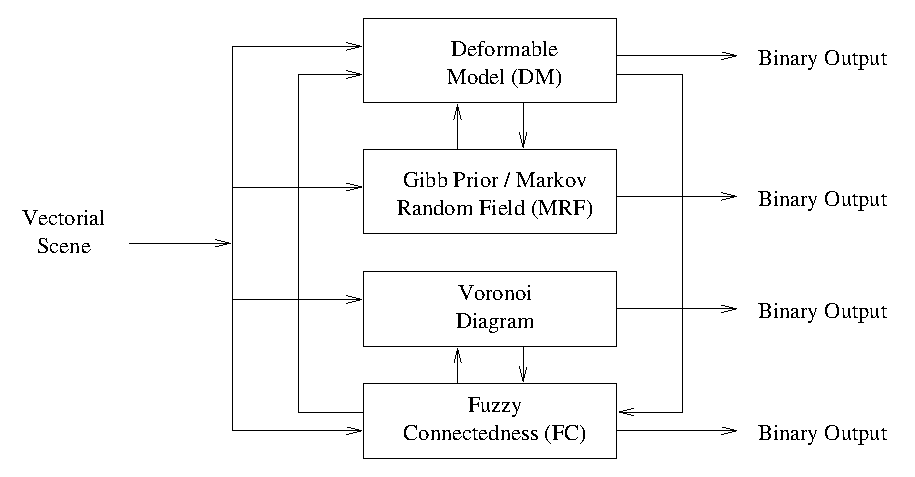
\includegraphics[width=6cm]{HybridSegmentationEngine1.eps}
\caption{Components of a HybridSegmentation approach}
\label{fig:HybridSegmentationEngine1}
\end{figure}

The Figure \ref{fig:HybridSegmentationEngine1} illustrates the main
components of the hybrid segmentation algorithm.

\begin{figure}
\center
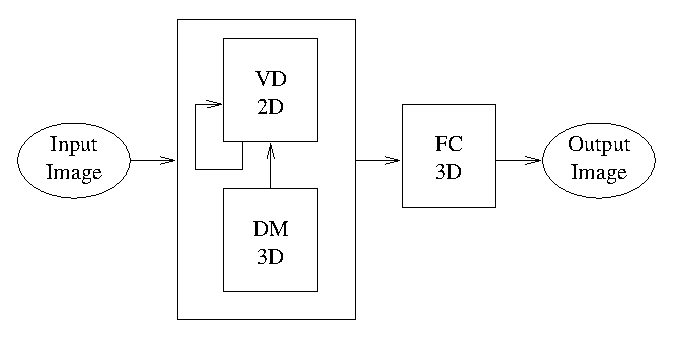
\includegraphics[width=6cm]{HybridSegmentationFCVDDM.eps}
\caption{Components of a HybridSegmentation approach}
\label{fig:HybridSegmentationFCVDDM}
\end{figure}


\begin{figure}
\center
\includegraphics[width=6cm]{VoronoiSegmentationClassDiagram1.eps}
\caption{UML Class Diagram of the VoronoiSegmentation filter}
\label{fig:VoronoiSegmentationClassDiagram1}
\end{figure}


\begin{figure}
\center
\includegraphics[width=6cm]{FuzzyConnectednessClassDiagram1.eps}
\caption{UML Class Diagram of the FuzzyConnectedness filter}
\label{fig:FuzzyConnectednessClassDiagram1}
\end{figure}


\begin{figure}
\center
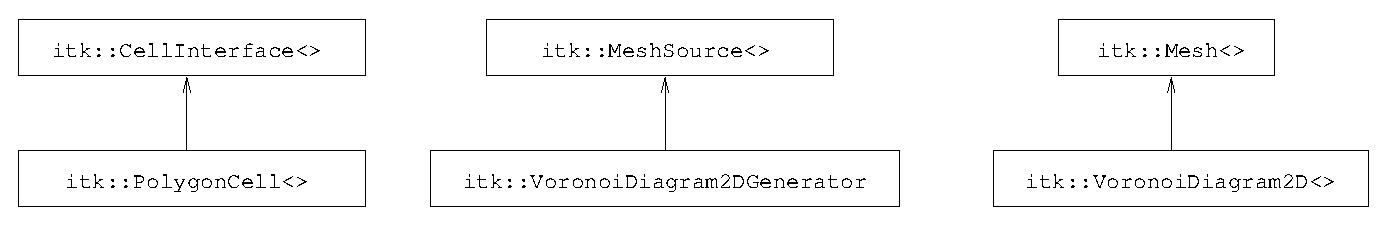
\includegraphics[width=6cm]{VoronoiSegmentationCollaborationDiagram1.eps}
\caption{UML Collaboration Diagram of the VoronoiSegmentation filter}
\label{fig:VoronoiSegmentationCollaborationDiagram1}
\end{figure}



\begin{figure}
\center
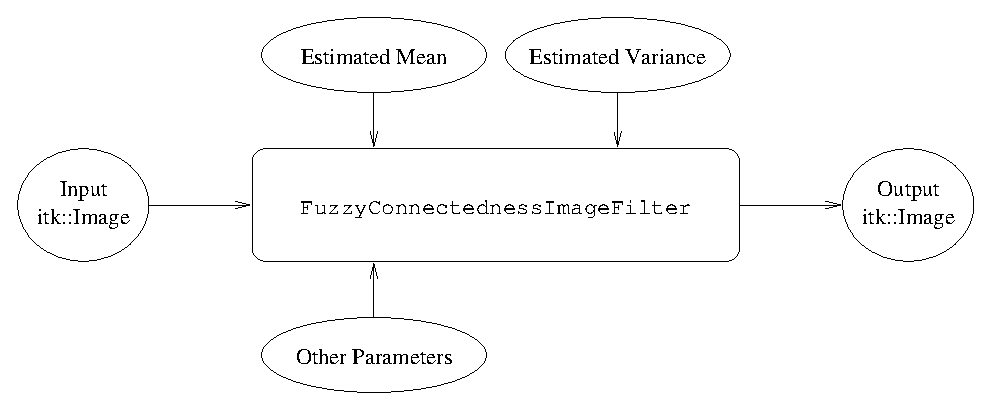
\includegraphics[width=6cm]{FuzzyConnectednessCollaborationDiagram1.eps}
\caption{UML Collaboration Diagram of the FuzzyConnectedness filter}
\label{fig:FuzzyConnectednessCollaborationDiagram1}
\end{figure}



\begin{figure}
\center
\includegraphics[width=6cm]{VoronoiSegmentationCollaborationDiagram2.eps}
\caption{UML Collaboration Diagram of the VoronoiSegmentation filter}
\label{fig:VoronoiSegmentationCollaborationDiagram2}
\end{figure}




\begin{figure}
\center
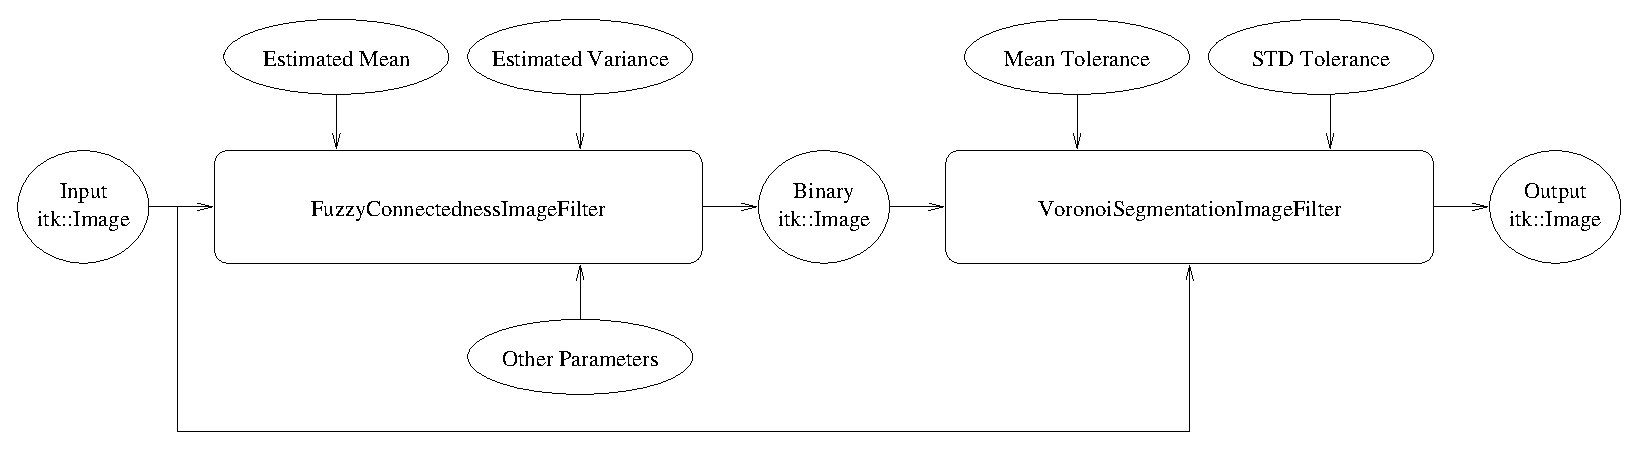
\includegraphics[width=6cm]{FuzzyVoronoiCollaborationDiagram1.eps}
\caption{UML Collaboration Diagram of the Fuzzy Voronoi Segmentation}
\label{fig:FuzzyVoronoiCollaborationDiagram1}
\end{figure}




\begin{figure}
\center
\includegraphics[width=6cm]{FuzzyVoronoiDeformableCollaborationDiagram1.eps}
\caption{UML Collaboration Diagram of the Fuzzy Voronoi Deformable Segmentation}
\label{fig:FuzzyVoronoiDeformableCollaborationDiagram1}
\end{figure}









%%%%%%%%%%%%%%%%%%%%%%%%%%%%%%%%%%%%%%%%%%%%%%%%%%%%%%%%%%%%%%%%%
%
%  Here is an example of how to include equations
%
%%%%%%%%%%%%%%%%%%%%%%%%%%%%%%%%%%%%%%%%%%%%%%%%%%%%%%%%%%%%%%%%%


\begin{equation}
MS(A,B) = \frac{1}{N} \sum_i^N \left( A_i - B_i \right)^2
\end{equation}





\subsection{Example}
\label{sec:HybridSegmentationExample1}

\input{HybridSegmentationFuzzyVoronoi.tex}



\fi



\chapter{Statistics}
\label{sec:StaisticsFramework}

This chapter introduces the statistics functionalities in Insight. The
statistics subsystem's primary purpose is to provide general capabilities
for statistical pattern classification. However, its use is not limited
for classification. Users might want to use data containers and
algorithms in the statistics subsystem to perform other statistical
analysis or to preprocessor image data for other tasks.

The statistics subsystem mainly consists of three parts: data container
classes, statistical algorithms, and the classification framework. In this
chapter, we will discuss each major part in that order.

\section{Data Containers}
\label{sec:StatisticsDataContainer}

An \subdoxygen{Statistics}{Sample} object is a data container of elements
that we call \emph{measurement vectors}. A measurement vector is an array of
values (of the same type) measured on an object (In images, it can be a
vector of the gray intensity value and/or the gradient value of a
pixel). Strictly speaking from the design of the Sample class, a measurement
vector can be any class derived from \doxygen{FixedArray}, including
FixedArray itself.

\begin{figure}
  \centering
  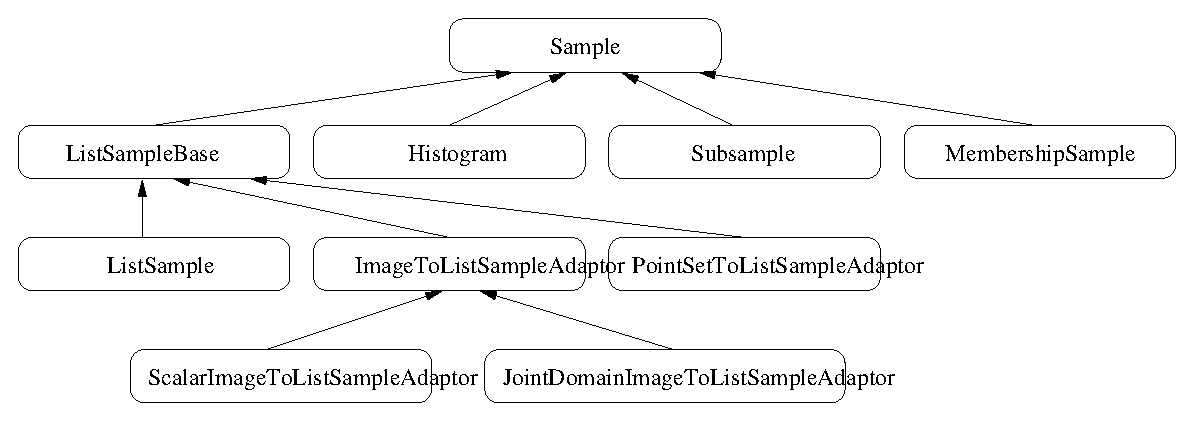
\includegraphics[width=0.9\textwidth]{SampleInheritanceTree.eps}
  \itkcaption[Sample class inheritance tree]{Sample class inheritance diagram.}
  \protect\label{fig:SampleInheritanceTree}
\end{figure}

\subsection{Sample Interface}
\label{sec:SampleInterface}

\ifitkFullVersion 
\input{ListSample.tex}
\fi

\subsection{Sample Adaptors}
\label{sec:SampleAdaptors}

There are two adaptor classes that provide the common
\subdoxygen{Statistics}{Sample} interfaces for \doxygen{Image} and
\doxygen{PointSet}, two fundamental data container classes found in ITK. The
adaptor classes do not store any real data elements themselves. These data
comes from the source data container plugged into them. First, we will
describe how to create an
\subdoxygen{Statistics}{ImageToListAdaptor} and then an
\subdoxygen{statistics}{PointSetToListAdaptor} object.

\subsubsection{ImageToListAdaptor}
\label{sec:ImageToListAdaptor}

\ifitkFullVersion 
\input{ImageToListAdaptor.tex}
\fi

\subsubsection{PointSetToListAdaptor}
\label{sec:PointSetToListAdaptor}

\ifitkFullVersion 
\input{PointSetToListAdaptor.tex}
\fi

\ifitkFullVersion 
\input{PointSetToAdaptor.tex}
\fi


\subsection{Histogram}
\label{sec:Histogram}

\ifitkFullVersion 
\input{Histogram.tex}
\fi

\subsection{Subsample}
\label{sec:Subsample}

\ifitkFullVersion 
\input{Subsample.tex}
\fi

\subsection{MembershipSample}
\label{sec:MembershipSample}

\ifitkFullVersion 
\input{MembershipSample.tex}
\fi

\subsection{MembershipSampleGenerator}
\label{sec:MembershipSampleGenerator}

\ifitkFullVersion 
\input{MembershipSampleGenerator.tex}
\fi


\subsection{K-d Tree}
\label{sec:KdTree}

\ifitkFullVersion 
\input{KdTree.tex}
\fi

\section{Algorithms and Functions}
\label{sec:StatisticsAlgorithmsFunctions}

In the previous section, we described the data containers in the ITK
statistics subsystem. We also need data processing algorithms and statistical
functions to conduct statistical analysis or statistical classification using
these containers. Here we define an algorithm to be an operation over a set
of measurement vectors in a sample. A function is an operation over
individual measurement vectors. For example, if we implement a class
(\subdoxygen{Statistics}{EuclideanDistance}) to calculate the Euclidean
distance between two measurement vectors, we call it a function, while if we
implemented a class (\subdoxygen{Statistics}{MeanCalculator}) to calculate
the mean of a sample, we call it an algorithm.

\subsection{Sample Statistics}
\label{sec:SampleStatistics}

We will show how to get sample statistics such as means and covariance from
the (\subdoxygen{Statistics}{Sample}) classes. Statistics can tells us
characteristics of a sample. Such sample statistics are very important for
statistical classification. When we know the form of the sample distributions
and their parameters (statistics), we can conduct Bayesian classification. In
ITK, sample mean and covariance calculation algorithms are implemented. Each
algorithm also has its weighted version (see Section
\ref{sec:WeightedMeanCovariance}). The weighted versions are used in the
expectation-maximization parameter estimation process.

\subsubsection{Mean and Covariance}
\label{sec:MeanCovariance}

\ifitkFullVersion 
\input{SampleStatistics.tex}
\fi

\subsubsection{Weighted Mean and Covariance}
\label{sec:WeightedMeanCovariance}

\ifitkFullVersion 
\input{WeightedSampleStatistics.tex}
\fi

\subsection{Sample Generation}
\label{sec:SampleGeneration}

\subsubsection{ListSampleToHistogramFilter}
\label{sec:ListSampleToHistogramFilter}

\ifitkFullVersion 
\input{ListSampleToHistogramFilter.tex}
\fi

\subsubsection{ListSampleToHistogramGenerator}
\label{sec:ListSampleToHistogramGenerator}

\ifitkFullVersion 
\input{ListSampleToHistogramGenerator.tex}
\fi

\subsubsection{NeighborhoodSampler}
\label{sec:NeighborhoodSampler}

\ifitkFullVersion 
\input{NeighborhoodSampler.tex}
\fi

\subsubsection{SampleToHistogramProjectionFilter}
\label{sec:SampleToHistogramProjectionFilter}

\ifitkFullVersion 
\input{SampleToHistogramProjectionFilter.tex}
\fi




\subsection{Sample Sorting}
\label{sec:SampleSorting}

\ifitkFullVersion 
\input{SampleSorting.tex}
\fi

\subsection{Probability Density Functions}
\label{sec:ProbabilityDensityFunctions}

The probability density function (PDF) for a specific distribution returns
the probability density for a measurement vector. To get the probability
density from a PDF, we use the \code{Evaluate(input)} method. PDFs for
different distributions require different sets of distribution
parameters. Before calling the \code{Evaluate()} method, make sure to set the
proper values for the distribution parameters.

\subsubsection{Gaussian Distribution}
\label{sec:GaussianDensityFunction}

\ifitkFullVersion 
\input{GaussianDensityFunction.tex}
\fi

\subsection{Distance Metric}
\label{sec:DistanceMetric}

\subsubsection{Euclidean Distance}
\label{sec:EuclideanDistance}

\ifitkFullVersion 
\input{EuclideanDistance.tex}
\fi

\subsection{Decision Rules}
\label{sec:DecisionRules}

A decision rule is a function that returns the index of one data element in a
vector of data elements. The index returned depends on the internal logic of
each decision rule. The decision rule is an essential part of the ITK
statistical classification framework. The scores from a set of membership
functions (e.g. probability density functions, distance metrics) are compared
by a decision rule and a class label is assigned based on the output of the
decision rule. The common interface is very simple. Any decision rule class
must implement the \code{Evaluate()} method. In addition to this method,
certain decision rule class can have additional method that accepts prior
knowledge about the decision task. The
\doxygen{MaximumRatioDecisionRule} is an example of such a class.

The argument type for the \code{Evaluate()} method is
\code{std::vector< double >}. The decision rule classes are part of the
\code{itk} namespace instead of \code{itk::Statistics} namespace.

For a project that uses a decision rule, it must link the \code{itkCommon}
library. Decision rules are not templated classes.

\subsubsection{Maximum Decision Rule}
\label{sec:MaximumDecisionRule}

\ifitkFullVersion 
\input{MaximumDecisionRule.tex}
\fi

\subsubsection{Minimum Decision Rule}
\label{sec:MinimumDecisionRule}

\ifitkFullVersion 
\input{MinimumDecisionRule.tex}
\fi

\subsubsection{Maximum Ratio Decision Rule}
\label{sec:MaximumRatioDecisionRule}

\input{MaximumRatioDecisionRule.tex}

\subsection{Random Variable Generation}
\label{sec:RandomVariableGeneration}

A random variable generation class returns a variate when the
\code{GetVariate()} method is called. When we repeatedly call the method
for ``enough'' times, the set of variates we will get follows
the distribution form of the random variable generation class.
 
\subsubsection{Normal (Gaussian) Distribution}
\label{sec:NormalVariateGeneration}

\ifitkFullVersion 
\input{NormalVariateGenerator.tex}
\fi


\section{Statistics applied to Images}
\label{sec:StatisticsAppliedToImages}

\subsection{Image Histograms}
\label{sec:ImageHistogram}


\subsubsection{Scalar Image Histogram with Adaptor}
\label{sec:ScalarImageHistogramAdaptor}
\ifitkFullVersion 
\input{ImageHistogram1.tex}
\fi


\subsubsection{Scalar Image Histogram with Generator}
\label{sec:ScalarImageHistogramGenerator}
\ifitkFullVersion 
\input{ImageHistogram2.tex}
\fi


\subsubsection{Color Image Histogram with Generator}
\label{sec:ColorImageHistogramGenerator}
\ifitkFullVersion 
\input{ImageHistogram3.tex}
\fi


\subsubsection{Color Image Histogram Writing}
\label{sec:ColorImageHistogramGeneratorWriting}
\ifitkFullVersion 
\input{ImageHistogram4.tex}
\fi


\subsection{Image Information Theory}
\label{sec:ComputingImageEntropy}

Many concepts from Information Theory have been used successfully in the domain
of image processing. This section introduces some of such concepts and
illustrates how the statistical framework in ITK can be used for computing
measures that have some relevance in terms of Information Theory
\cite{Shannon1948,Shannon1949,Kullback1997}.


\subsubsection{Computing Image Entropy}
\label{sec:ComputingImageEntropy}

\index{Entropy!What's wrong in images}

The concept of Entropy has been introduced into image processing as a crude
mapping from its application in Communications. The notions of Information
Theory can be decepting and misleading when applied to images because their
language from Communication Theory does not necessarily maps to what people in
the Imaging Community use.

For example, it is commonly said that

\emph{``The Entropy of an image is a measure of the amount of information
contained in an image''}. 

This statement is fundamentally \textbf{incorrect}. 

The way the notion of Entropy is commonly measured in images is by first
assuming that the spatial location of a pixel in an image is irrelevant!  That
is, we simply take the statistical distribution of the pixel values as it can
be evaluated in a histogram and from that histogram we estimate the frequency
of the value associated to each bin. In other words, we simply assume that the
image is a set of pixels that are passing through a channel, just as things are
commonly considered for communication purposes.

Once the frequency of every pixel value has been estimated, Information Theory
defines that the amount of uncertainty that an observer will lose by taking one
pixel and finding its real value to be the one associated with the i-th bin of the
histogram, is given by $-\log_2{(p_i)}$, where $p_i$ is the frequency in that
histogram bin. Since a reduction in uncertainty is equivalent to an increase in
the amount of information in the observer, we conclude that measuring one pixel
and finding its level to be in the i-th bin results in an acquisition of
$-\log_2{(p_i)}$ bits of information\footnote{Note that \textbf{bit} is the unit of
amount of information. Our modern culture has vulgarized the bit and its
multiples, the Byte, KiloByte, MegaByte, GigaByte and so on as simple measures
of the amount of RAM memory and capacity of a hard drive in a computer. In that
sense, a confusion is created between the encoding of a piece of data and its
actual amount of information. For example a file composed of one million
letters will take one million bytes in a hard disk, but it does not necessariy
has one million bytes of information, since in many cases parts of the file can
be predicted from others. This is the reason why data compression can manage to
compact files.}.

Since we could have picked any pixel at random, our chances or picking the ones
that are associated to the i-th histogram bin are given by $p_i$. Therefore,
the expected reduction in uncertainty that we can get from measuring the value
of one pixel is given by

\begin{equation}
H = - \sum_i{ p_i  \cdot \log_2{(p_i)} }
\end{equation}

This quantity $H$ is what is usually defined as the \emph{Entropy of the
Image}. It would be more accurate to call it the Entropy of the random variable
associated to the intensity value of \emph{one} pixel. The fact that $H$ is
unrelated to the spatial arrangement of the pixels in an image shows how little
of the real \emph{Image Information} is $H$ actually representing. The Entropy
of an image, as mesure above, is only a crude indication of how the intensity
values are spread in the dynamic range of intensites. For example, an image
with maximum entropy will be the one that has a large dynamic range and every
value in that range is equally probable. 

The common acceptation of $H$ as a representation of image information has
terribly undermined the enormous potential on the application of Information
Theory to image processing and analysis.

The real concepts of Information Theory would require that we define the amount
of information in an image based on our expectations and prior knowledge from
that image. In particular, the \emph{Amount of Information} provided by an
image should measure the number of features that we are not able to predict
based on our prior knowledge about that image. For example, if we know that we
are going to analyze a CT scan of the abdomen of an adult human male in the age
range of 40 to 45, there is already a good deal that we could predict about the
content of that image.  The real amount of information in the image is the
representation of the features in the image that we could not predict from
knowing that it is a CT scan from a human adult male.

The application of Information Theory to image analysis is still in its early
infancy and it is an exciting an promising field to be explored further. All
that being said, let's now look closer at how the concept of Entropy (which is
not the amount of information in an image) can be measured with the ITK
statistics framework.

\ifitkFullVersion 
\input{ImageEntropy1.tex}
\fi

\subsubsection{Computing Images Mutual Information}
\label{sec:ComputingImagesMutualInformation}

\ifitkFullVersion 
\input{ImageMutualInformation1.tex}
\fi



\section{Classification}
\label{sec:Classification}

In statistical classification, each object is represented by $d$ features (a
measurement vector), and the goal of classification becomes finding compact and
disjoint regions (decision regions\cite{Duda2000}) for classes in a
$d$-dimensional feature space. Such decision regions are defined by decision
rules that are known or can be trained.  The simplest configuration of a
classification consists of a decision rule and multiple membership functions;
each membership function represents a class. Figure~\ref{fig:simple}
illustrates this general framework.

\begin{figure}[h]
  \centering
  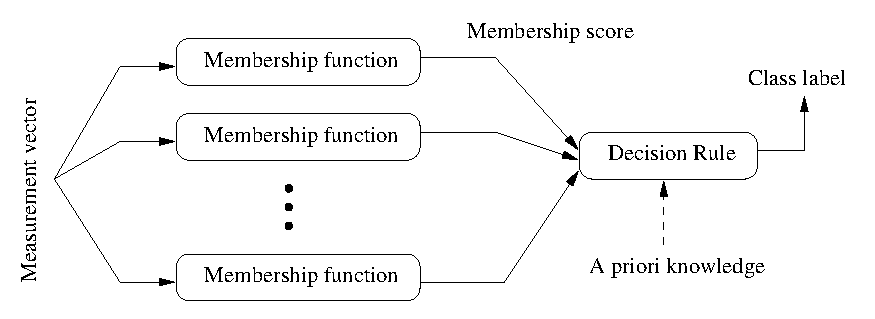
\includegraphics[width=0.7\textwidth]{DudaClassifier.eps}
  \itkcaption[Simple conceptual classifier]{Simple conceptual classifier.}
  \label{fig:simple}
\end{figure}

This framework closely follows that of Duda and
Hart\cite{Duda2000}. The classification process can be described
as follows:

\begin{enumerate}
\item{A measurement vector is input to each membership function.}
\item{Membership functions feed the membership scores to the
    decision rule.}
\item{A decision rule compares the membership scores and returns a
    class label.}
\end{enumerate}

\begin{figure}
  \centering
  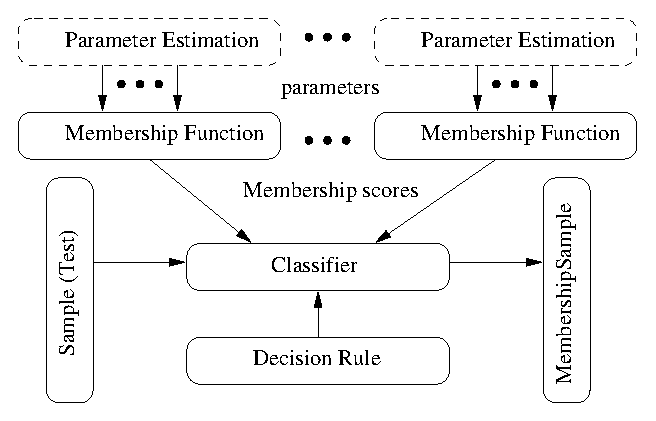
\includegraphics[width=0.7\textwidth]{StatisticalClassificationFramework.eps}
  \itkcaption[Statistical classification framework]{Statistical classification
framework.}
  \protect\label{fig:StatisticalClassificationFramework}
\end{figure}

This simple configuration can be used to formulated various classification
tasks by using different membership functions and incorporating task specific
requirements and prior knowledge into the decision rule. For example, instead
of using probability density functions as membership functions, through
distance functions and a minimum value decision rule (which assigns a class
from the distance function that returns the smallest value) users can achieve a
least squared error classifier. As another example, users can add a rejection
scheme to the decision rule so that even in a situation where the membership
scores suggest a ``winner'', a measurement vector can be flagged as ill
defined. Such a rejection scheme can avoid risks of assigning a class label
without a proper win margin.

\subsection{k-d Tree Based k-Means Clustering}
\label{sec:KdTreeBasedKMeansClustering}
\ifitkFullVersion
\input{KdTreeBasedKMeansClustering.tex}
\fi

\subsection{K-Means Classification}
\label{sec:KMeansClassifier}
\ifitkFullVersion
\input{ScalarImageKmeansClassifier.tex}
\fi

\subsection{Bayesian Plug-In Classifier}
\label{sec:BayesianPluginClassifier}

\ifitkFullVersion 
\input{BayesianPluginClassifier.tex}
\fi


\subsection{Expectation Maximization Mixture Model Estimation}
\label{sec:ExpectationMaximizationMixtureModelEstimation}

\ifitkFullVersion 
\input{ExpectationMaximizationMixtureModelEstimator.tex}
\fi

\subsection{Classification using Markov Random Field}
\label{sec:MarkovRandomField}

Markov Random Fields are probabilistic models that use the correlation between
pixels in a neighborhood to decide the object region. The
\subdoxygen{Statistics}{MRFImageFilter} uses the maximum a posteriori (MAP)
estimates for modeling the MRF. The object traverses the data set and uses the
model generated by the Mahalanobis distance classifier to gets the the distance
between each pixel in the data set to a set of known classes, updates the
distances by evaluating the influence of its neighboring pixels (based on a MRF
model) and finally, classifies each pixel to the class which has the minimum
distance to that pixel (taking the neighborhood influence under consideration).
The energy function minimization is done using the iterated coditional modes
(ICM) algorithm \cite{Besag1986}.

\ifitkFullVersion
\input{ScalarImageMarkovRandomField1.tex}
\fi 





\backmatter

%%%%%%%%%%%%%%%%%%%%%%%%%%%%%%%%%%%%%%%%%
%
%  Insert the bibliography using BibTeX
%
%%%%%%%%%%%%%%%%%%%%%%%%%%%%%%%%%%%%%%%%%

\bibliographystyle{plain}
\bibliography{\bibtexdatabasepath}


%%%%%%%%%%%%%%%%%%%%%%%%%%%%%%%%%%%%%%%%%
%
%  Insert the Index file
%
%%%%%%%%%%%%%%%%%%%%%%%%%%%%%%%%%%%%%%%%%

\printindex


%\ifitkPrintedVersion
%\cleardoublepage
%\newpage
\thispagestyle{empty}
\includegraphics[width=14cm]{flyer-activiz.eps}
\newpage
\thispagestyle{empty}
\includegraphics[width=14cm]{flyer-cmake.eps}
\newpage
\thispagestyle{empty}
\includegraphics[width=14cm]{flyer-itk.eps}
\newpage
\thispagestyle{empty}
\includegraphics[width=14cm]{flyer-kitware.eps}
\newpage
\thispagestyle{empty}
\includegraphics[width=14cm]{flyer-paraview.eps}
\newpage
\thispagestyle{empty}
\includegraphics[width=14cm]{flyer-polyviz.eps}
\newpage
\thispagestyle{empty}
\includegraphics[width=14cm]{flyer-volview.eps}
\newpage
\thispagestyle{empty}
\includegraphics[width=14cm]{flyer-vtk-textbook.eps}

%\fi

\end{document}
